\chapter{Experiments}
\label{Experiments}

In this chapter we describe experiment results based on methodology stated in Chapter~\ref{Methodology}. We use ITOP dataset \parencite{haque_towards_2016} for comparison with different models. To compare our results with existing models we use as a reference such models: RF \parencite{shotton_real-time_2011}, RTW \parencite{ho_yub_jung_random_2015}, IEF \parencite{carreira_human_2016}, VI \parencite{haque_towards_2016}, REN \parencite{chen_pose_2020}, Pose-net \parencite{moon_v2v-posenet_2018}, all of which were overviewed in Chapter~\ref{Related work}.

In Section~\ref{s:one-stage-training} we show our results with one stage straining scheme compared to the two-stage described in Section~\ref{s:one-stage-network-training}.

In Section~\ref{s:results-on-itop} we show the performance of the one-stage training model on the ITOP dataset \parencite{haque_towards_2016}. Also, we compare our results with state-of-the-art models for the same task.

In Section~\ref{s:experiment-noise} we show a comparison of models' performance on a dataset with additional noise described in Section-\ref{s:how-noise-affects-models-performance}. As a reference model we use SOTA model - Pose-net \parencite{moon_v2v-posenet_2018}.

In Section~\ref{s:experiment-lack-of-data} we compare our proposed model with the SOTA Pose-net model with truncated dataset size to assess models' convergence.

% -------------------------- Experiment setup -------------------------
\section{Experiment setup}
\label{s:experiment-setup}
In this section, we describe the basic setup for our experiments. Some experiments have additional changes to the training/evaluation pipelines described in dedicated subsections.

All experiments were performed on a server with 8 CPU core, 1 GPU card Nvidia Tesla P100 (16.2 Gb of video memory), and 60 Gb of RAM. As a training framework, Pytorch 1.8.1 was used based on CUDA 10.1 video driver. This setup was powered by the Google Colab backend.

All point clouds from the ITOP dataset were preprocessed according to Section~\ref{Data-preparation}. For threshold filtering and normalization we use NumPy Python library, and for point cloud clusterization and human extraction we use C++ PCL \parencite{noauthor_strawlabpython-pcl_2021} library with Python bindings. After preprocessing we reduce the number of points in the human cloud to 2,000 to speed up the model's training time. The Adam optimizer \parencite{kingma_adam_2017} was used for all experiments. The initial learning rate is $lr = 10^{-4}$ with learning rate decay of $10^{-1}$ each $30$ epochs. The average number of epoch to a fully trained model is $~80$, after this time of epoch our model starts to oscillate on the plateau. The average training time in such a setup is 16 machine hours. The batch size of $12$ was used. After each epoch of the training dataset, we run evaluation pipelines to measure the model's performance, on each evaluation run we save such metrics: reconstruction loss (Formula~\ref{eqn:chamfer-distance}), regression loss (Formula~\ref{eqn:regression-loss}), total loss (Formula~\ref{eqn:aggregated-loss}), mAP for $10\  cm$ distance (Formula~\ref{eqn:dataset-metric-map}). For visualization purposes, we also save input and reconstructed point clouds ($P$ and $\hat{P}$ accordingly).


% -------------------------- ONE STAGE TRAIN -------------------------
\section{Effectiveness of one stage training}
\label{s:one-stage-training}
In this section, we compare our proposed approach of a one-stage training scheme with the original two-stage one \parencite{wu_3d_2020}.

The main objective of one-stage training is to reduce the number of hyperparameters and speed up training via aggregation strategy of reconstruction and regression losses in the network. There are two experiments conducted on the original architecture described by \cite{wu_3d_2020} and our proposed method described in Section~\ref{s:one-stage-network-training}.

At first, we train capsule networks with a two-stage setup. For the first stage, we use the setup described in Section~\ref{s:experiment-setup} and freeze the regression part of the network, thus we train only the reconstruction part. In this setup, we run 70 epochs and save the model. The second stage uses weights of the model from the first step, but now freeze feature extractor and reconstruction parts of the network and train only regression. In this setup, only 20 epochs are needed to fully converge.

The second experiment adopts our proposed solution with loss aggregation. In this experiment, we train all the networks at once, without freezing any layers. This experiment is done according to Section~\ref{s:experiment-setup}.

The comparison of the two experiments is shown in Table~\ref{tab:two-stage-vs-one-stage}. 

\begin{table}[H]
    \caption{The comparison of one stage and two stage training pipeline (based on Formula~\ref{eqn:dataset-metric-map} metric)}
    \label{tab:two-stage-vs-one-stage}
    \centering
    \begin{tabular}{l l l l}
    \toprule
    \tabhead{Dataset} & \tabhead{Two stage training} & \tabhead{One state training (our method)} & \tabhead{Difference} \\
    \midrule
    ITOP front view & 79.6\%  & 83.1\%  & 3.5\% \\
    ITOP side view & 70.8\% & 74.2\%  & 3.4\% \\
    \bottomrule\\
    \end{tabular}
\end{table}


\begin{figure}[!htbp]
    \centerline{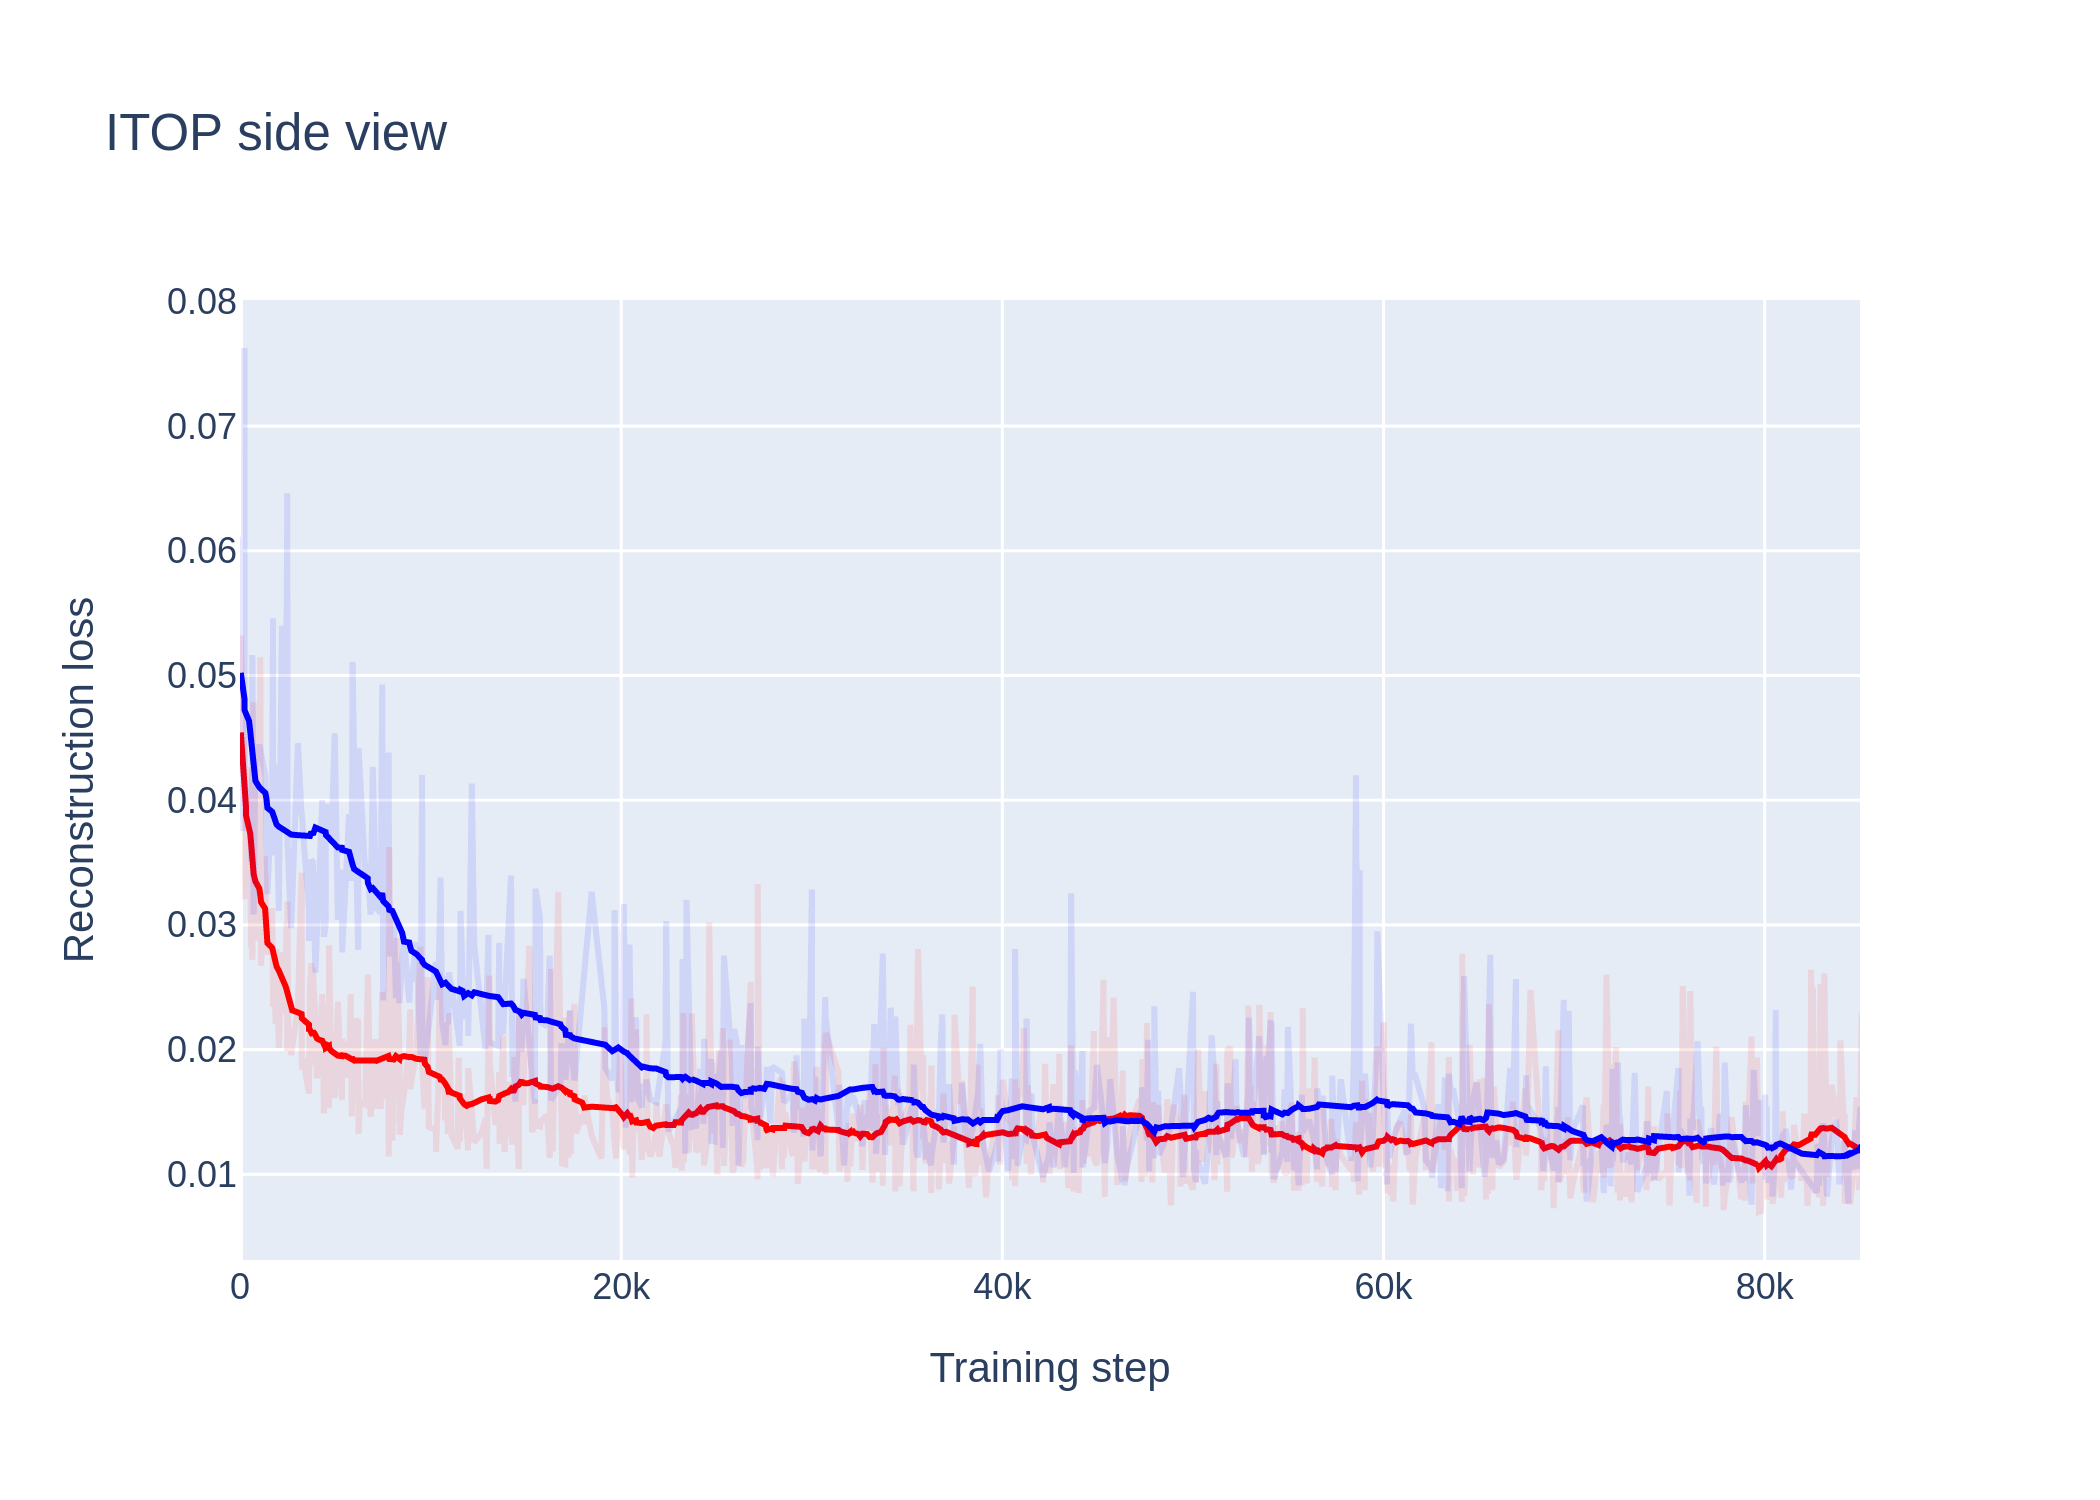
\includegraphics[scale=0.15]{Figures/one-stage-vs-two-stage.png}}
    \caption{Reconstruction loss function for two stage (red) model and one stage model(blue)}
    \label{img:one-stage-vs-two-stage-reconstruction}
\end{figure}

\begin{figure}[htbp]
    \centerline{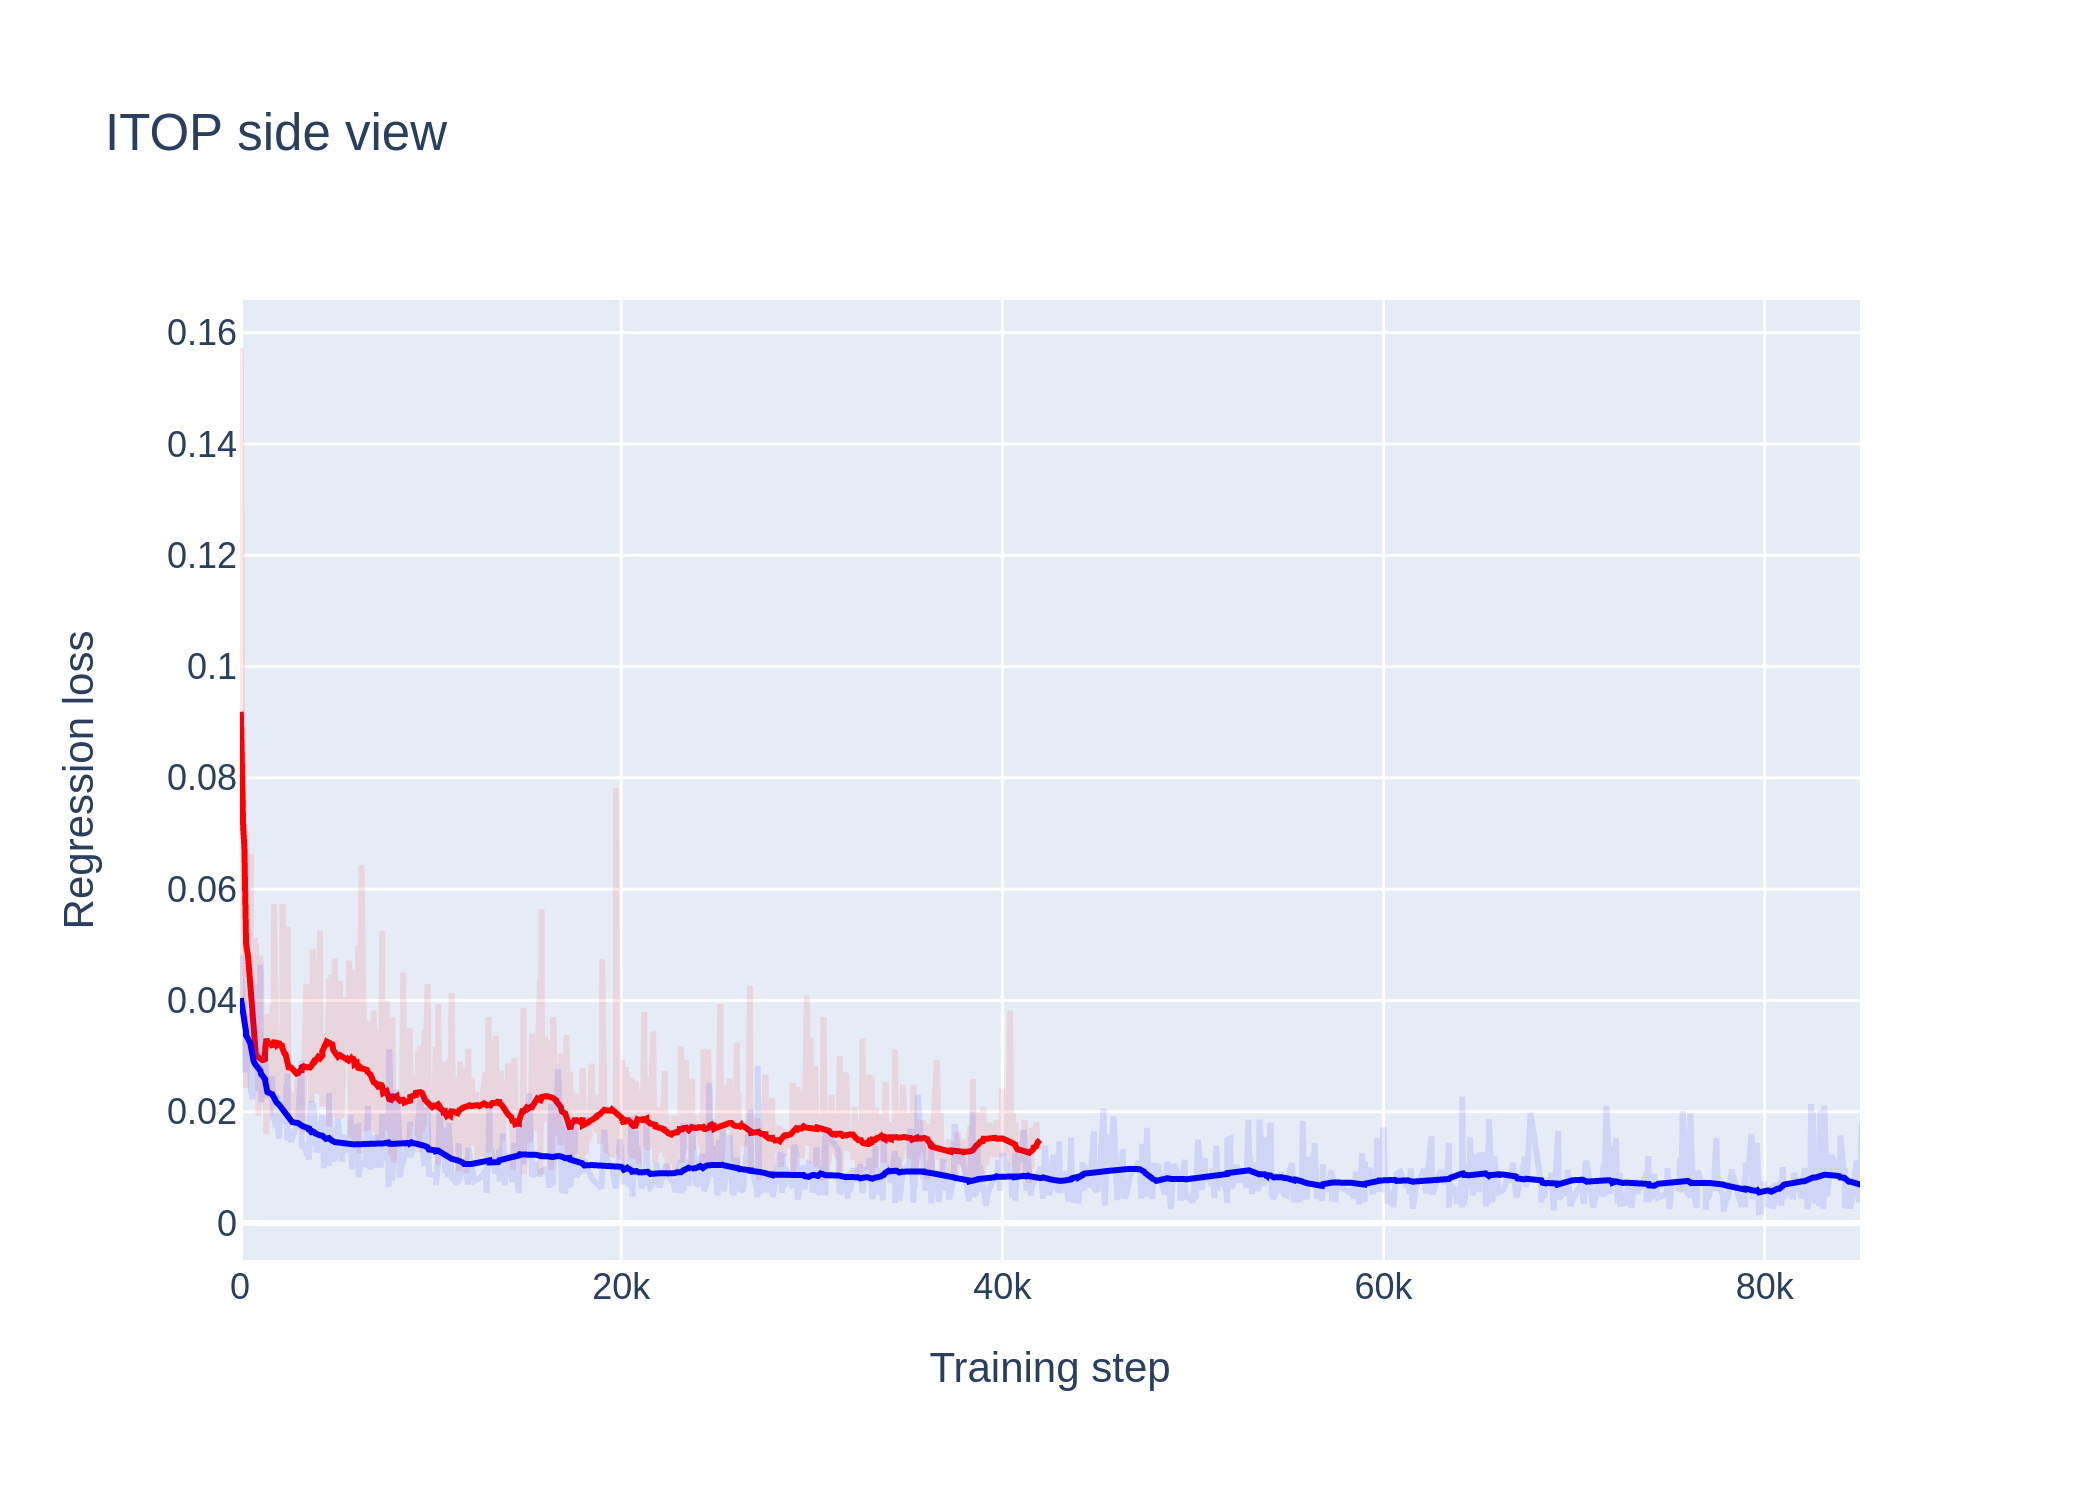
\includegraphics[scale=0.15]{Figures/one-stage-vs-two-stage-regression.png}}
    \caption{Regression loss function for two stage (red) model and one stage model(blue)}
    \label{img:one-stage-vs-two-stage-regression}
\end{figure}

\begin{figure}[htbp]
    \centerline{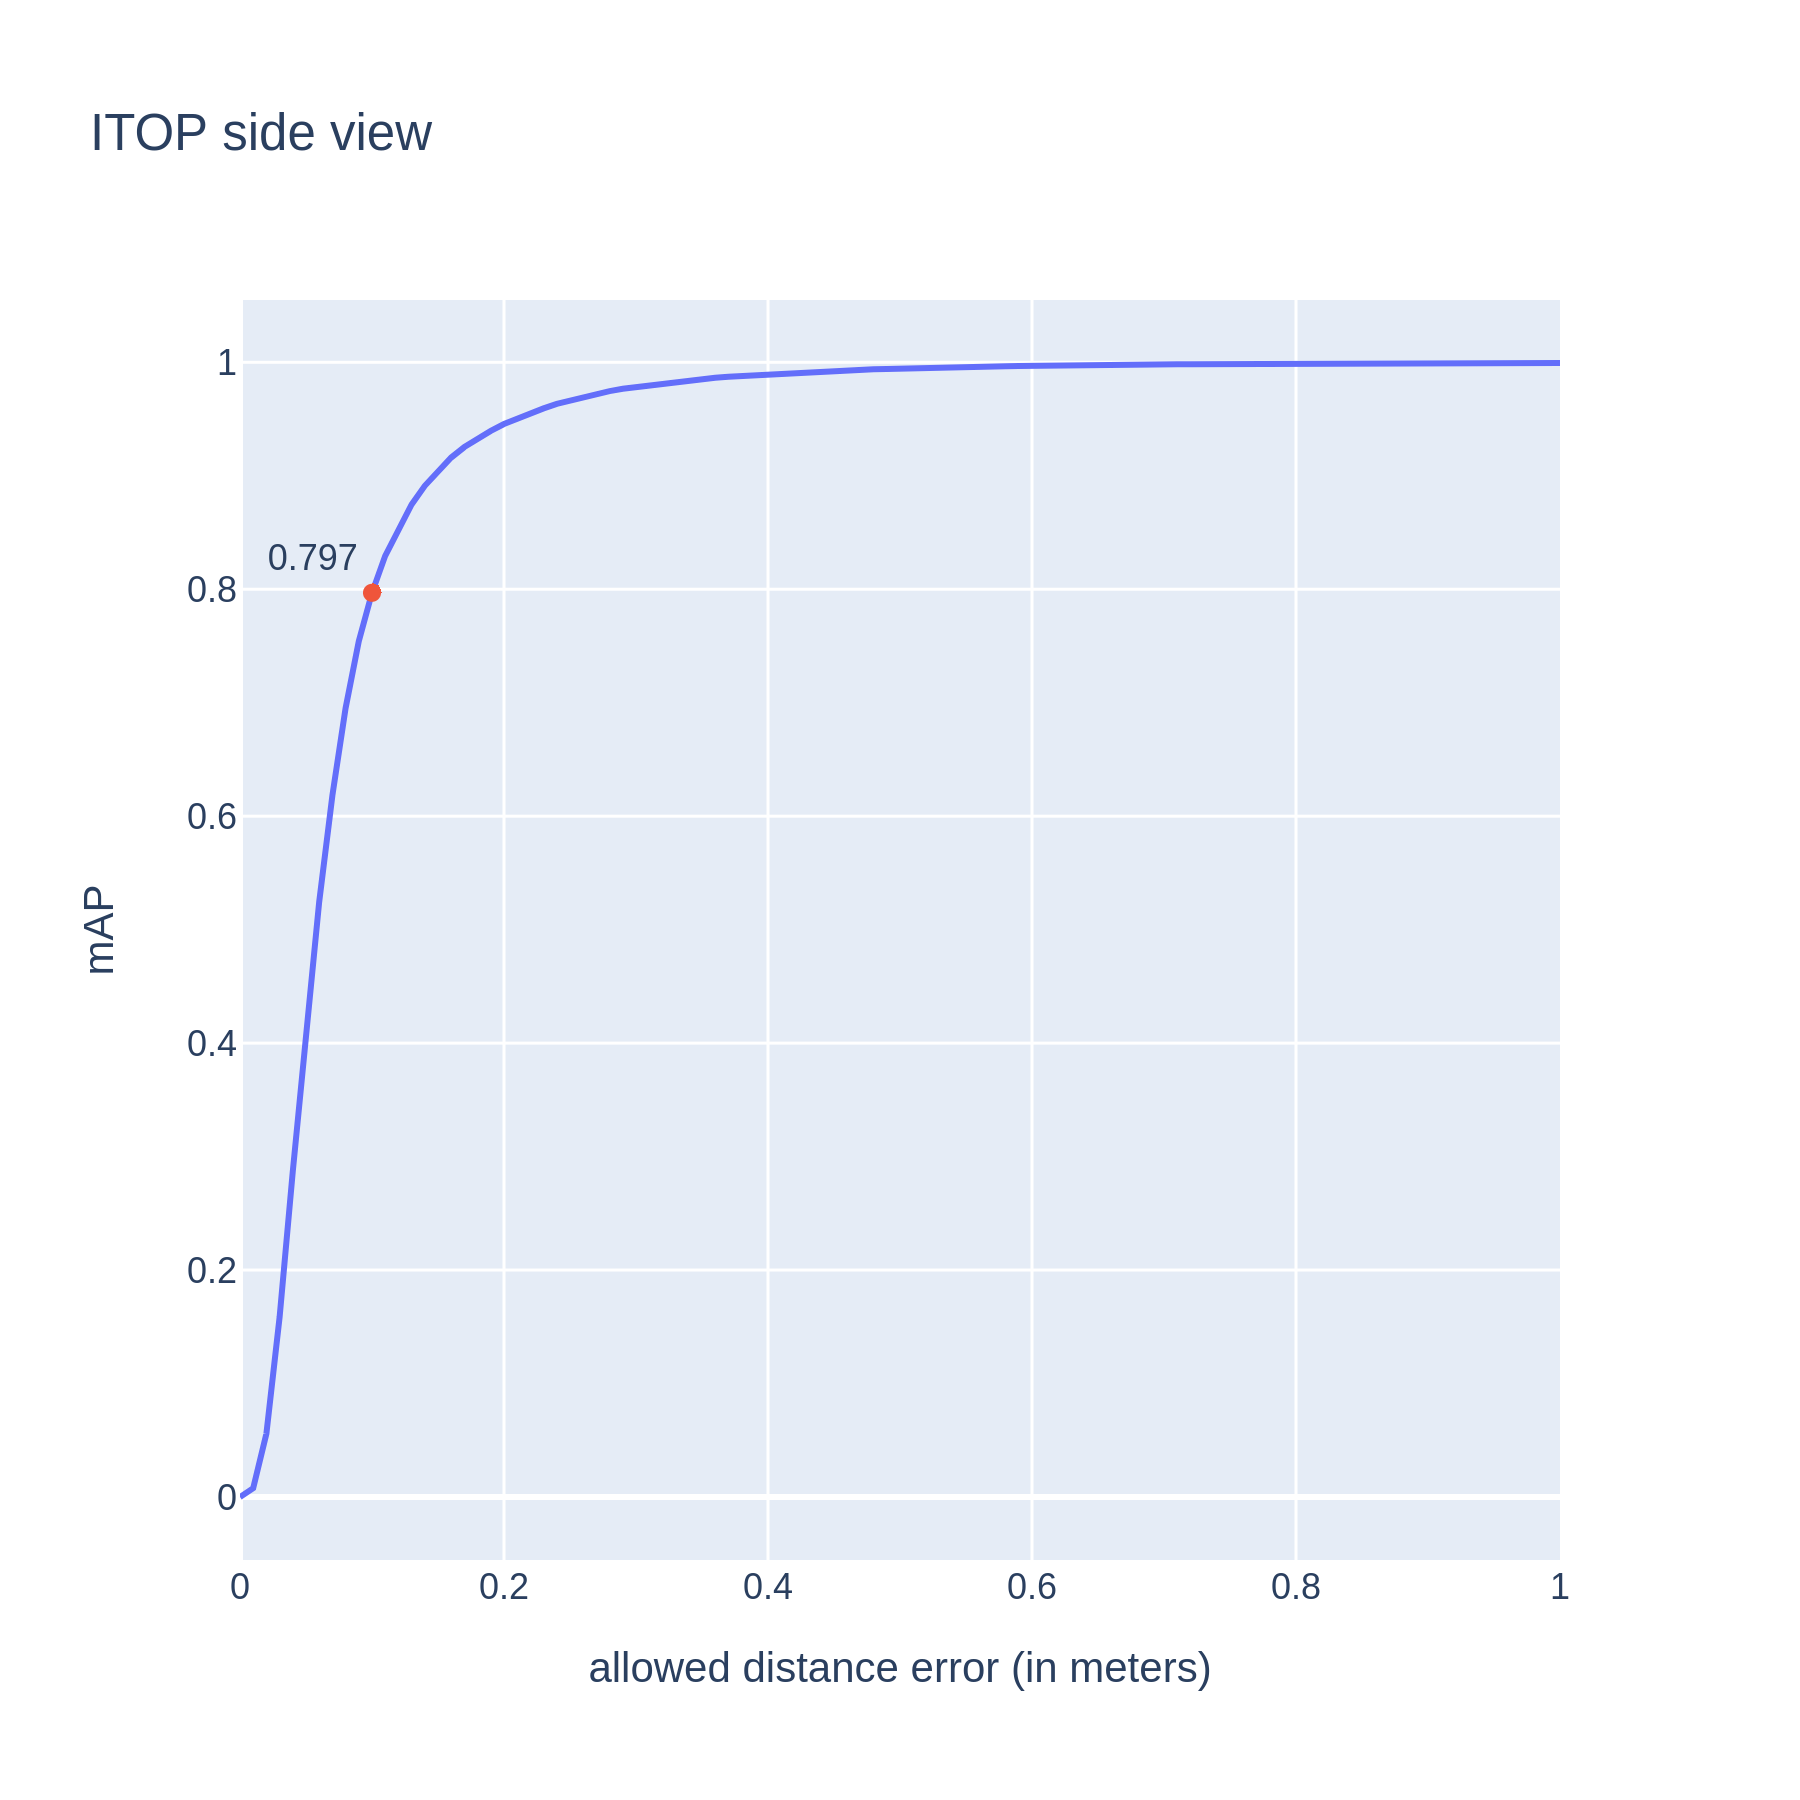
\includegraphics[trim=50 100 50 100,clip,scale=0.15]{Figures/two-stage-map.png}}
    \caption{Two stage model for side view. mAP for different distance errors for two stage model. 10 cm distance mAP is highlighted}
    \label{img:two-stage-map}
\end{figure}

\begin{figure}[htbp]
    \centerline{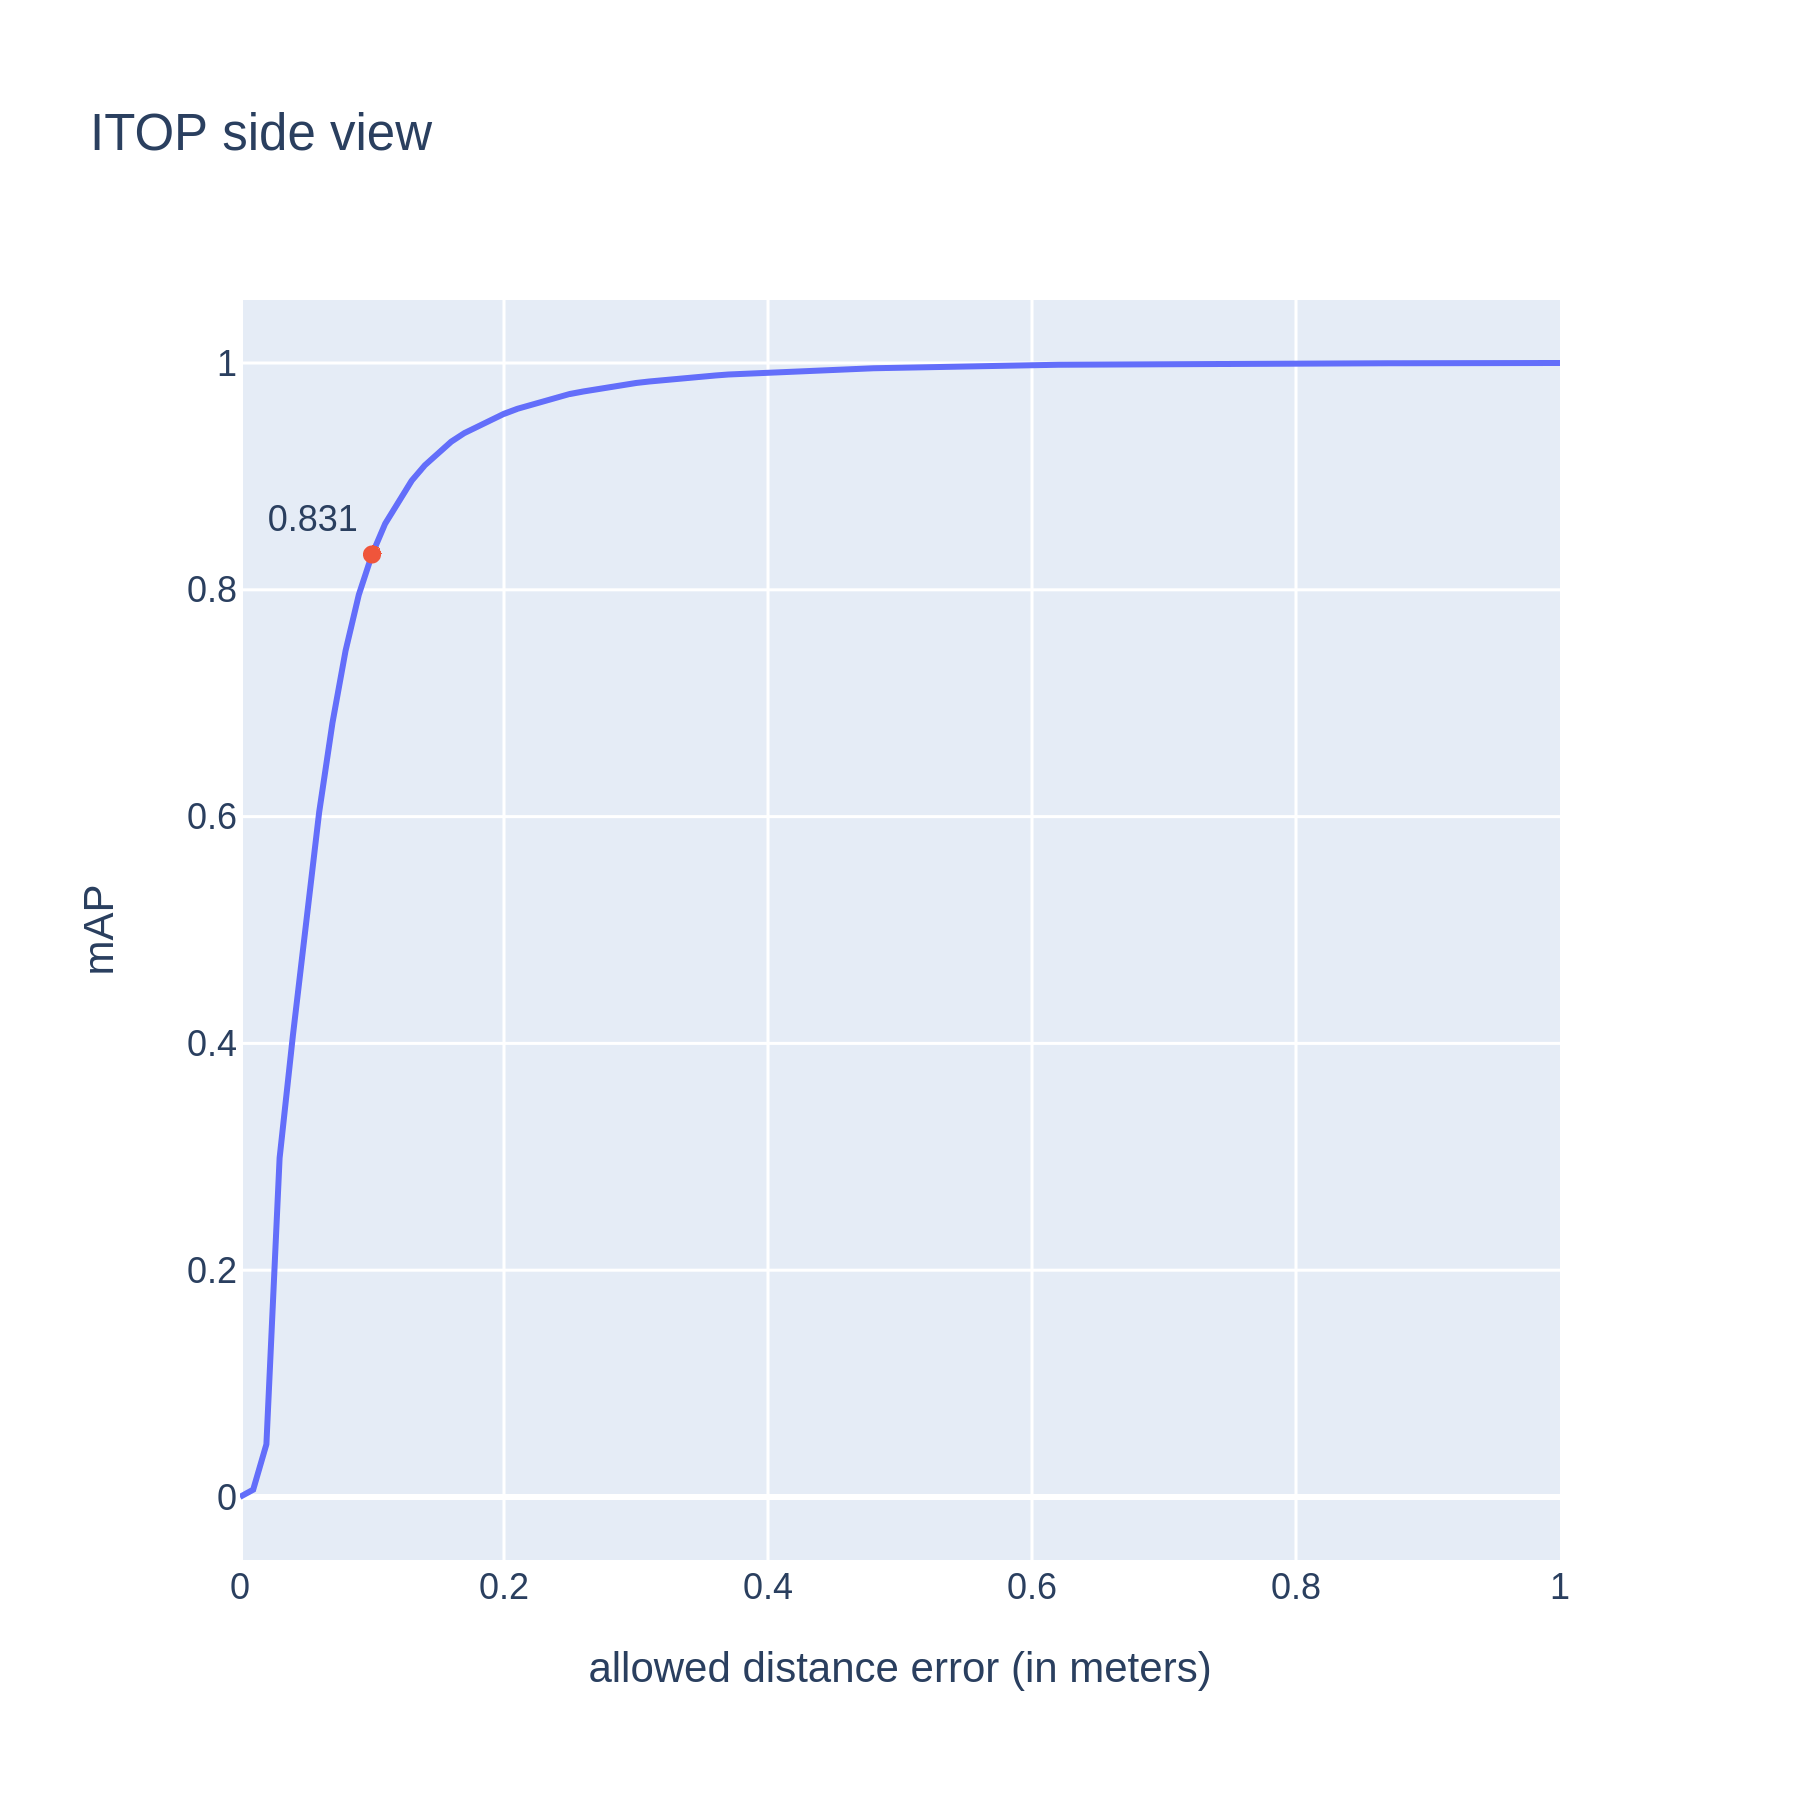
\includegraphics[trim=50 100 50 100,clip,scale=0.15]{Figures/one-stage-map.png}}
    \caption{One stage model for side view. mAP for different distance errors for two stage model. 10 cm distance mAP is highlighted}
    \label{img:one-stage-map}
\end{figure}


\begin{figure}[htbp]
    \centerline{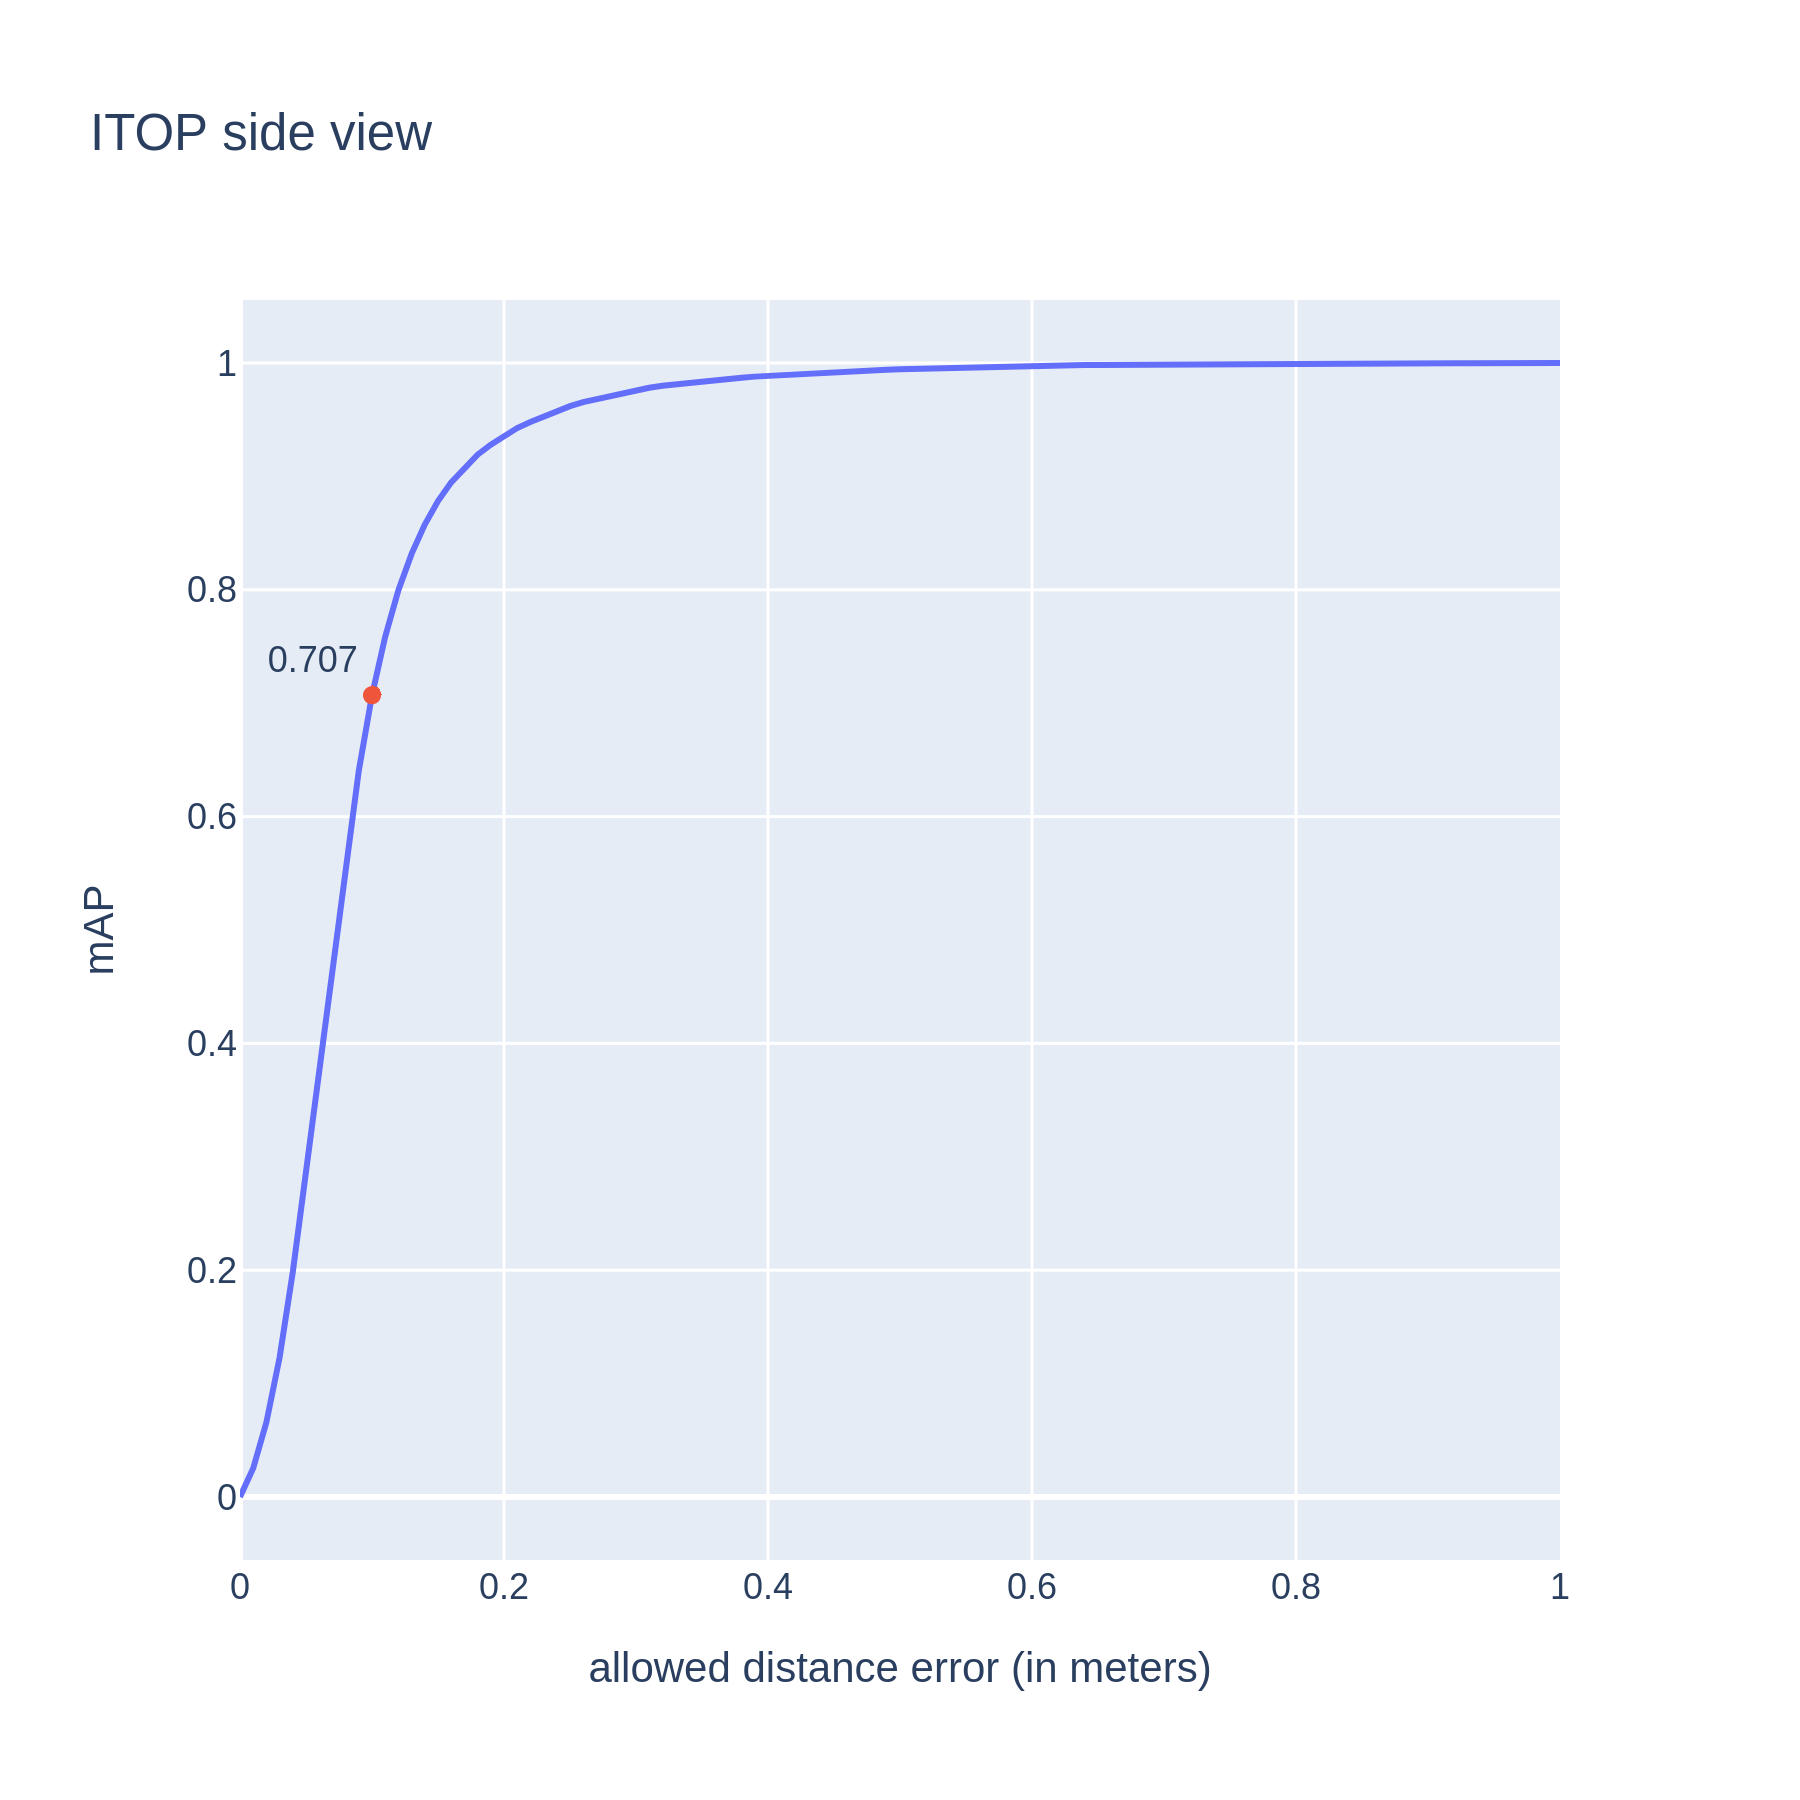
\includegraphics[trim=50 100 50 100,clip,scale=0.15]{Figures/two-stage-map-top-view.png}}
    \caption{Two stage model for top view. mAP for different distance errors for two stage model. 10 cm distance mAP is highlighted}
    \label{img:two-stage-map-side-view}
\end{figure}

\begin{figure}[htbp]
    \centerline{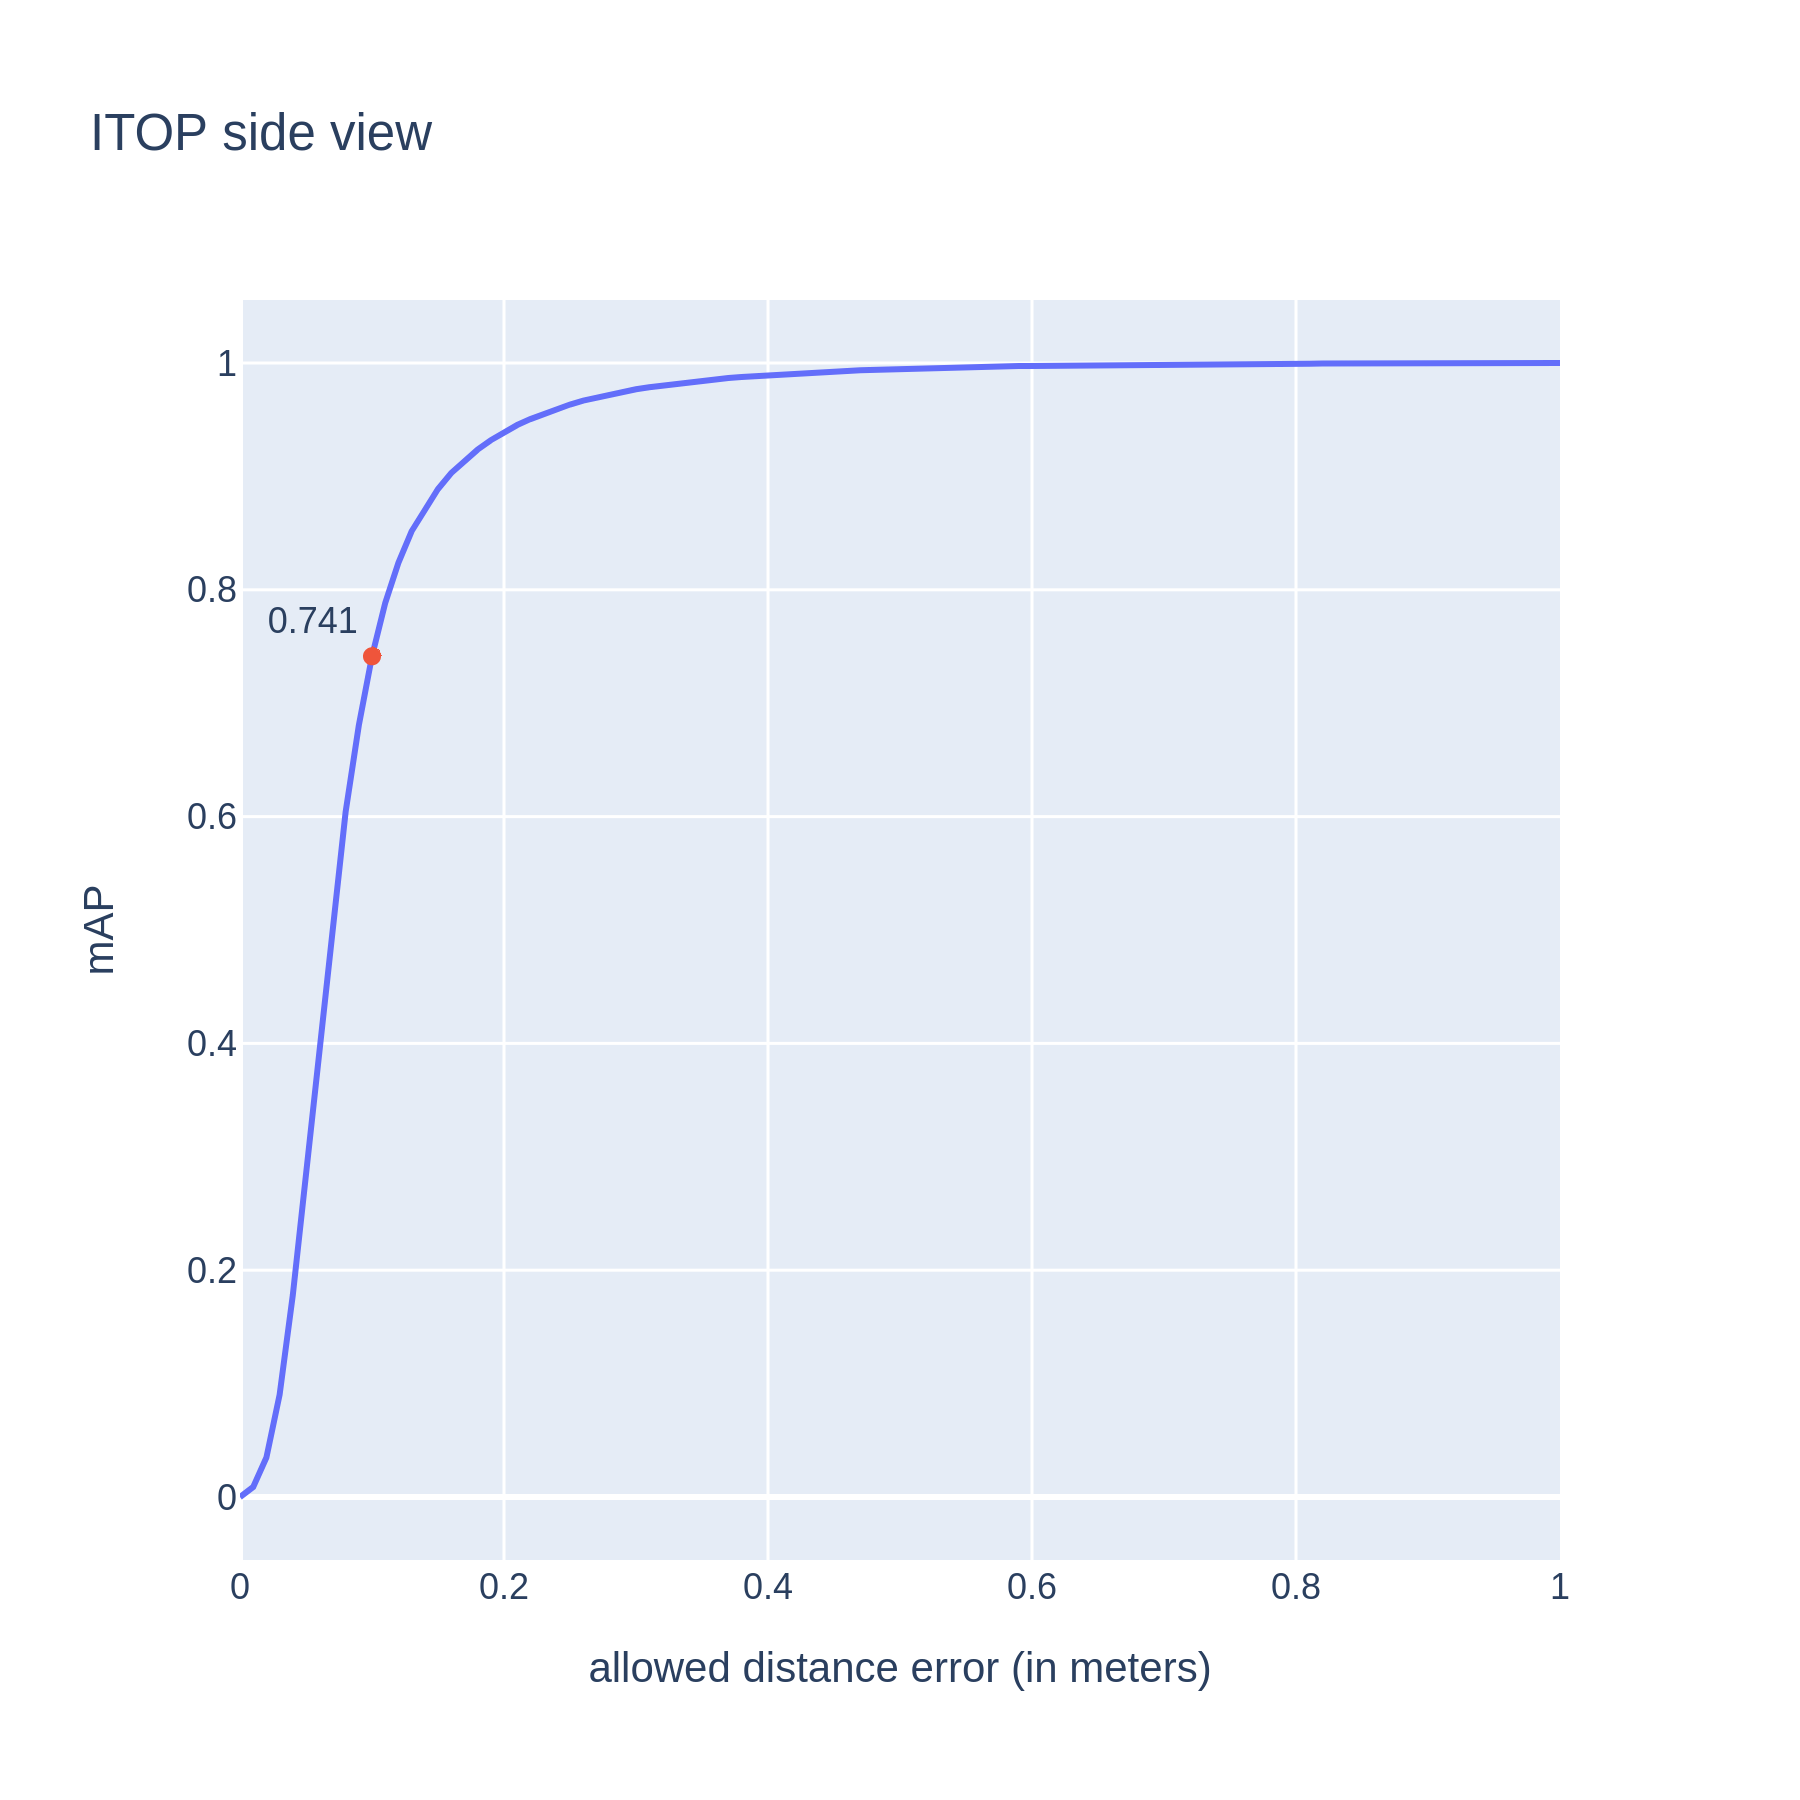
\includegraphics[trim=50 100 50 100,clip,scale=0.15]{Figures/one-stage-map-top-view.png}}
    \caption{One stage model for top view. mAP for different distance errors for two stage model. 10 cm distance mAP is highlighted}
    \label{img:one-stage-map-side-view}
\end{figure}

% -------------------------- ITOP DATASET -------------------------
\section{Results on ITOP dataset}
\label{s:results-on-itop}

We have conducted training and evaluation of our capsule-based model on the ITOP dataset (side and top views). The results of the evaluation, as well as the performance of SOTA models, are shown in Table~\ref{tab:itop-side-view} for side view, and in Table~\ref{tab:itop-top-view} for top view.

\begin{table}
    \caption{Comparison of proposed model with SOTA models on ITOP side view dataset}
    \label{tab:itop-side-view}
    \centering
    \begin{tabular}{l|cccccc|c}
    \hline & \multicolumn{6}{|c} { mAP (side-view) } \\
    \hline Body part & RF & RTW & IEF & VI & REN-9x6x6 & PoseNet & Our model \\
    \hline Head & $63.8$ & $97.8$ & $96.2$ & $98.1$ & $98.7$ & $98.29$ & $94.7$\\
    Neck & $86.4$ & $95.8$ & $85.2$ & $97.5$ & $99.4$ & $99.07$ & $96.9$ \\
    Shoulders & $83.3$ & $94.1$ & $77.2$ & $96.5$ & $96.1$ & $97.18$ & $93.7$ \\
    Elbows & $73.2$ & $77.9$ & $45.4$ & $73.3$ & $74.7$ & $80.42$ & $73.9$ \\
    Hands & $51.3$ & $70.5$ & $30.9$ & $68.7$ & $55.2$ & $67.26$ & $58.0$ \\
    Torso & $65.0$ & $93.8$ & $84.7$ & $85.6$ & $98.7$ & $98.73$ & $97.0$ \\
    Hip & $50.8$ & $80.3$ & $83.5$ & $72.0$ & $91.8$ & $93.23$ & $89.5$ \\
    Knees & $65.7$ & $68.8$ & $81.8$ & $69.0$ & $89.0$ & $91.80$ & $88.1$ \\
    Feet & $61.3$ & $68.4$ & $80.9$ & $60.8$ & $81.1$ & $87.6$ & $80.0$ \\
    \hline Mean & $65.8$ & $80.5$ & $71.0$ & $77.4$ & $84.9$ & $88.74$ & $83.1$ \\
    \hline
    \end{tabular}
\end{table}

\begin{table}
    \caption{Comparison of proposed model with SOTA models on ITOP top view dataset}
    \label{tab:itop-top-view}
    \centering
    \begin{tabular}{l|cccccc|c}
    \hline & \multicolumn{6}{|c} { mAP (top-view) } \\
    \hline Body part & RF & RTW & IEF & VI & REN-9x6x6 & PoseNet & Our model \\
    \hline Head & $95.4$ & $98.4$ & $83.8$ & $98.1$ & $98.2$ & $98.4$ & $94.2$ \\
     Neck & $98.5$ & $82.2$ & $50.0$ & $97.6$ & $98.9$ & $98.91$ & $96.0$ \\
     Shoulders & $89.0$ & $91.8$ & $67.3$ & $96.1$ & $96.6$ & $9 6.87$ & $89.2$ \\
     Elbows & $57.4$ & $80.1$ & $40.2$ & $86.2$ & $74.4$ & $79.16$ & $67.6$ \\
     Hands & $49.1$ & $76.9$ & $39.0$ & $85.5$ & $50.7$ & $62.44$ & $48.9$ \\
     Torso & $80.5$ & $68.2$ & $30.5$ & $72.9$ & $98.1$ & $97.78$ & $94.0$ \\
     Hip & $20.0$ & $55.7$ & $38.9$ & $61.2$ & $85.5$ & $86.91$ & $79.3$ \\
     Knees & $2.6$ & $53.9$ & $54.0$ & $51.6$ & $70.0$ & $8 3.28$ & $80.3$ \\
     Feet & $0.0$ & $28.7$ & $62.4$ & $51.5$ & $41.6$ & $69.62$ & $67.4$ \\
    \hline Mean & $47.4$ & $68.2$ & $51.2$ & $75.5$ & $75.5$ & $83.44$ & $74.1$ \\
    \hline
    \end{tabular}
\end{table}

Our proposed model shows competitive results both on ITOP side view and front view. Our model outperforms RF \parencite{shotton_real-time_2011}, RTW \parencite{ho_yub_jung_random_2015}, IEF \parencite{carreira_human_2016} models on both datasets, and aslo VI \parencite{haque_towards_2016} on side-view only. The model still underperform REN \parencite{chen_pose_2020}, Pose-net \parencite{moon_v2v-posenet_2018} models.

Our model gives good results on head, neck, shoulders, torso body parts, and struggle to estimate hands and feet. It's difficult for a model to predict a key joint that is located in a relatively small point cloud (compared to whole-body).


In the Figure~\ref{img:reconstruction-example} we could see how the model reconstructs the human body with each epoch. On first epochs, the model outputs just a random point cloud, and with each new epoch, it trains to reproduce the input point cloud. As we can see from $d)$ in Figure~\ref{img:reconstruction-example} on epoch 60 the model's approximation is pretty solid.

\begin{figure}[htbp]
    \centerline{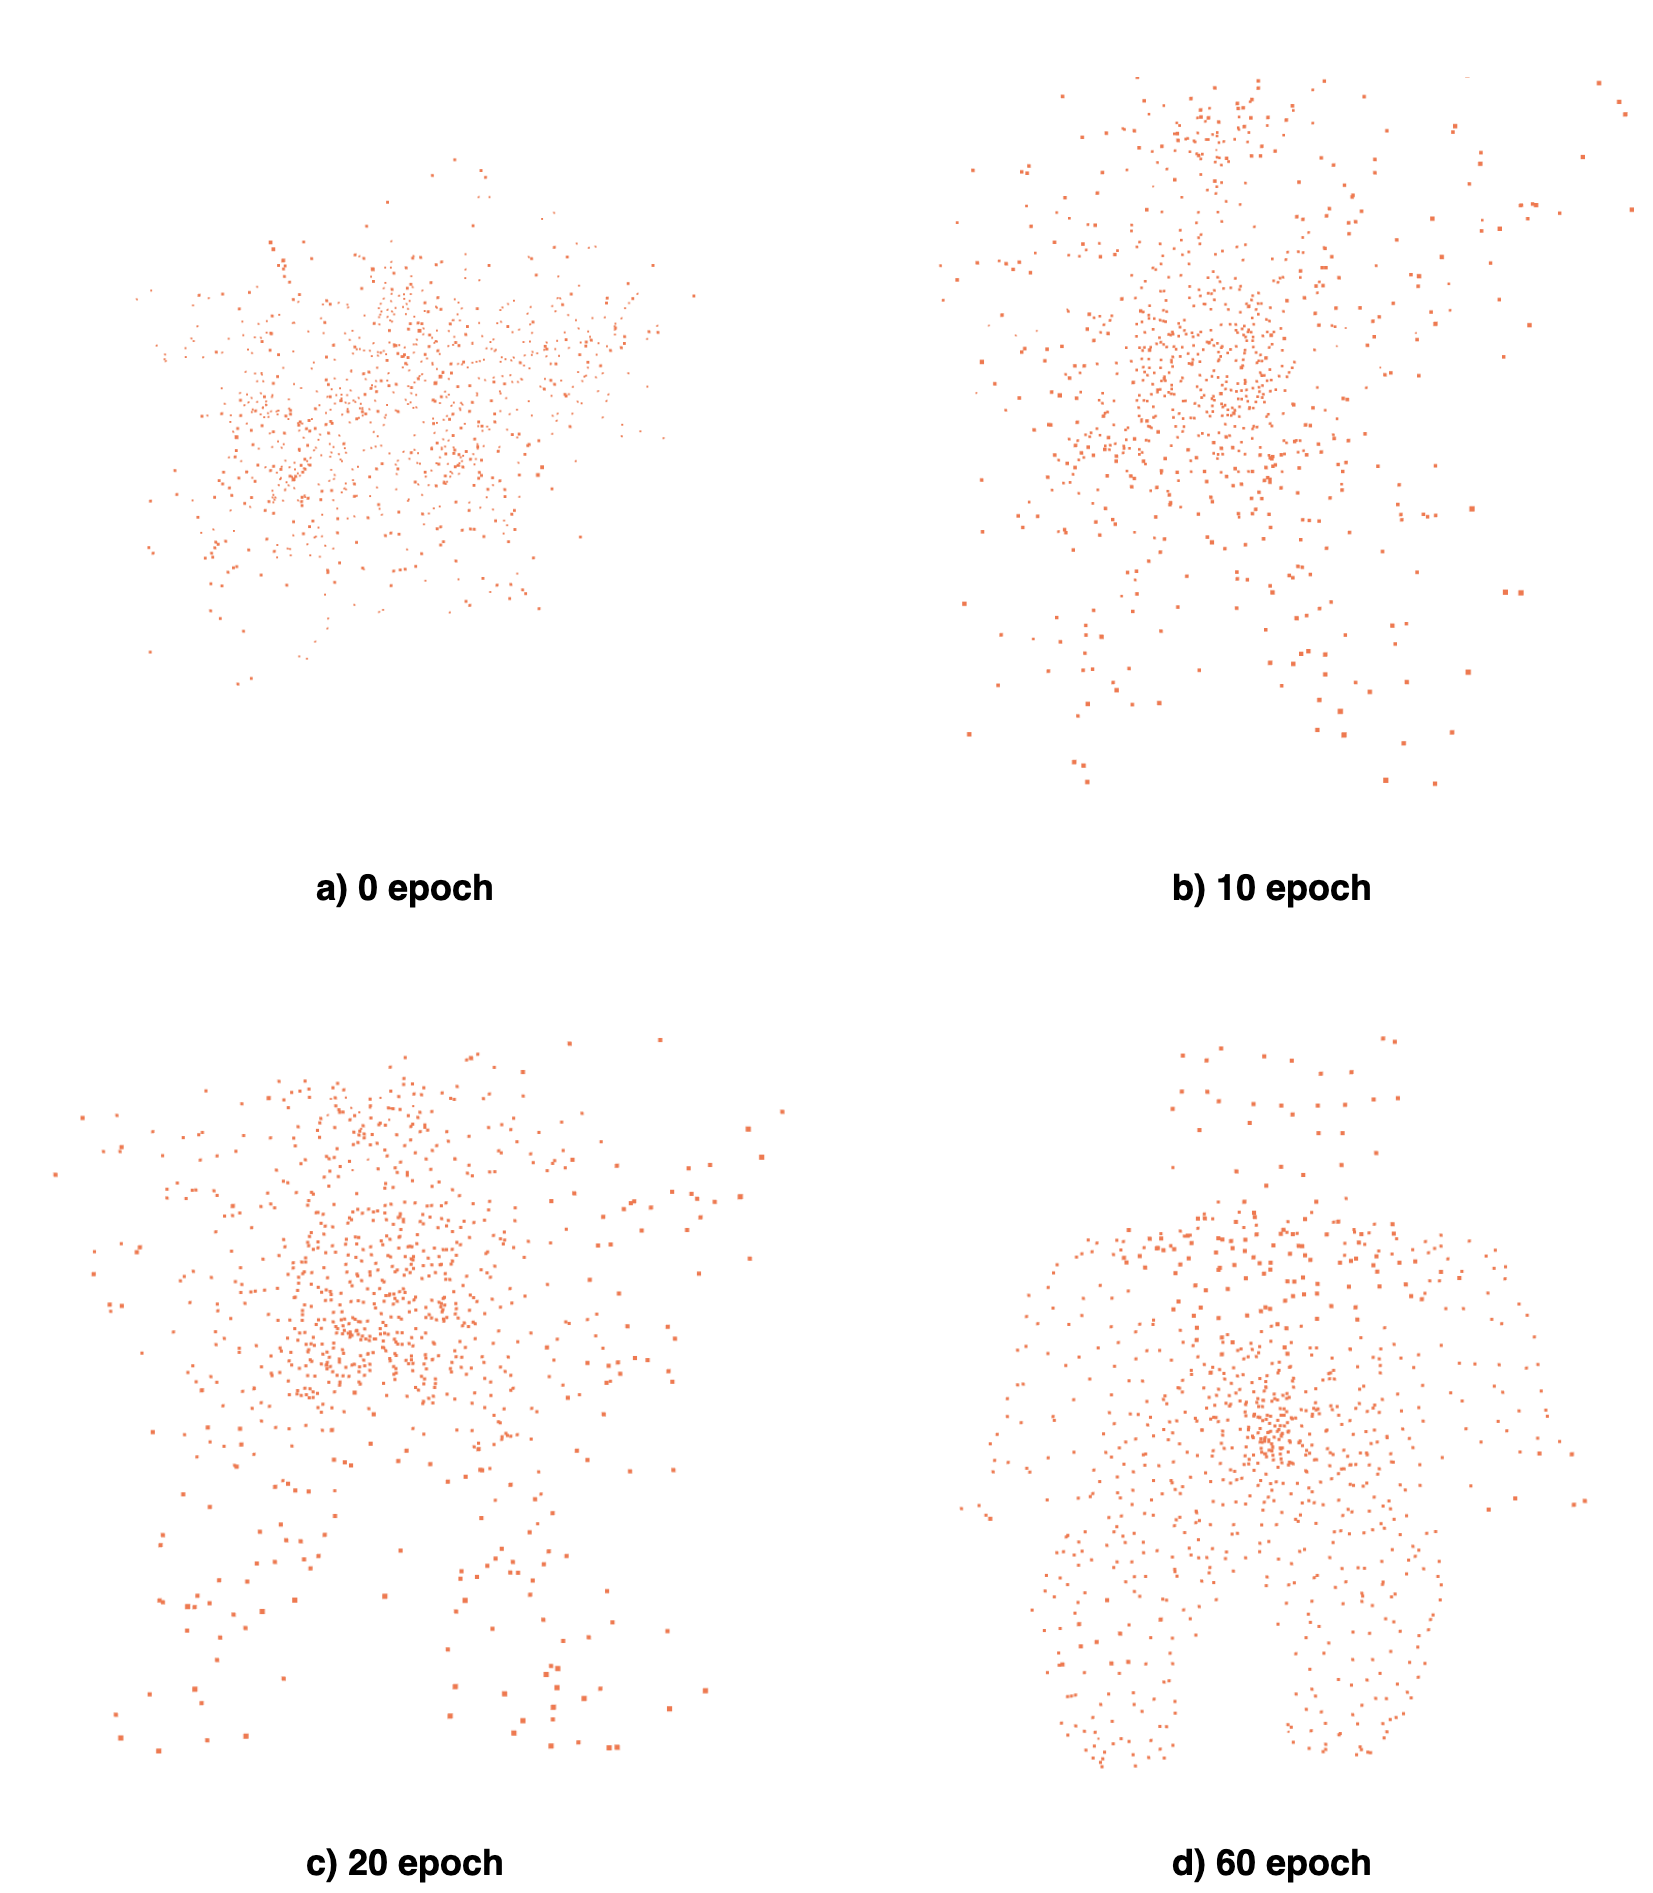
\includegraphics[scale=0.25]{Figures/reconstruction-example.png}}
    \caption{One stage model for top view. mAP for different distance errors for two stage model. 10 cm distance mAP is highlighted}
    \label{img:reconstruction-example}
\end{figure}

% -------------------------- NOISE IN DATA -------------------------

\section{How noise affects models' performance}
\label{s:experiment-noise}

In this section, we evaluate a capsule-based model (proposed solution) and a reference model (PoseNet) on a dataset with a different amount of noise. The experiment's description is covered in Section~\ref{s:how-noise-affects-models-performance}.

We use Gaussian noise and uniform noise as a mixin to the initial data. For the Gaussian noise, we add noise with a probability of $\frac{1}{3}$ (to roughly 30\% of points). We use two types of values for $\sigma$ - $0.1$ for mild noise and $0.2$ for more aggressive.

For uniform distribution we use constant number of additional points $N_P = 300$. That is roughly $15\%$ of additional points out of mean human point cloud size.
In Figure~\ref{img:human-with-noisy-data} is shown an example of human point clouds with additional noise. We don't add noise to ground truths key joints.

\begin{figure}[htbp]
    \centerline{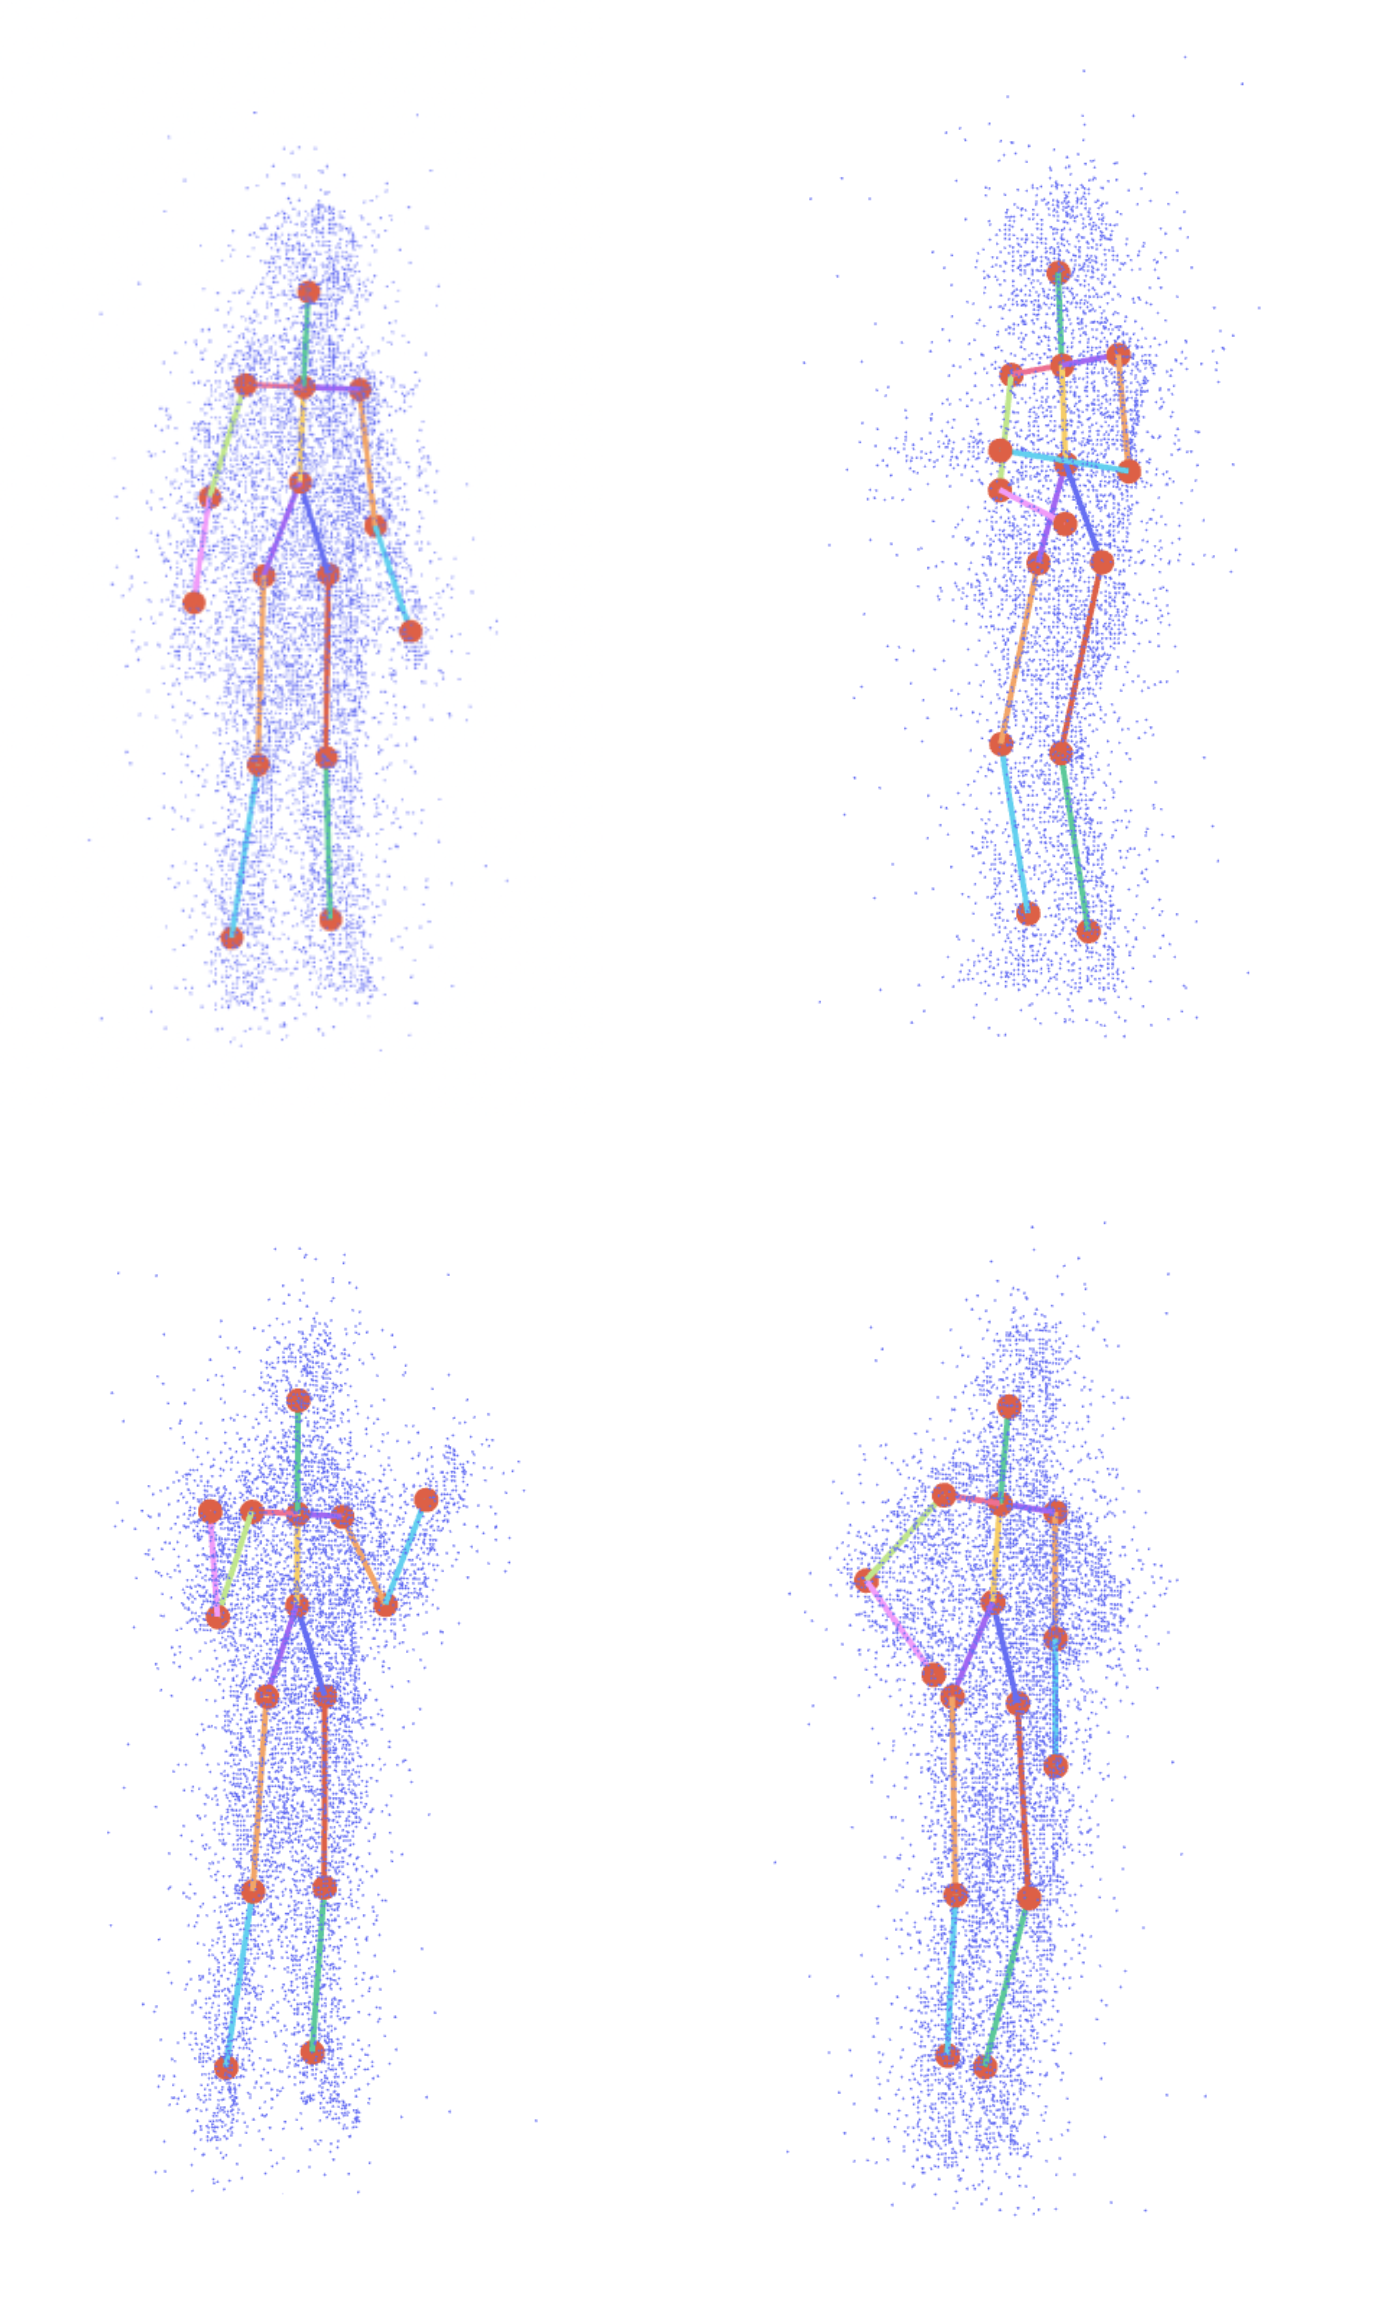
\includegraphics[scale=0.18]{Figures/human-with-noise.png}}
    \caption{Example of human points clouds with added noise. $\sigma - 0.1$, $N_P = 300$}
    \label{img:human-with-noisy-data}
\end{figure}

As for the capsule-based model we use the model trained on the ITOP side view dataset from the Experiment~\ref{s:results-on-itop}. We will use the ITOP side view dataset as a benchmark for this experiment.

As for reference model we use pretrained\footnote{\url{https://github.com/mks0601/V2V-PoseNet_RELEASE}} PoseNet.

We inference the ITOP side view dataset with different noise parameters for both models and measure mAP for each experiment. All experiments are collected in Table~\ref{tab:noise-table-comparison}.

\begin{table}[H]
    \caption{The comparison of capsnet model and PoseNet on dataset with different amount of noise on ITOP side view dataset}
    \label{tab:noise-table-comparison}
    \centering
    \begin{tabular}{l l l l l}
    \toprule
    \tabhead{Noise setup} & \tabhead{PoseNet} & \tabhead{CapsNet} & \tabhead{PoseNet difference} & \tabhead{CapsNet difference}  \\
    \midrule
    No noise (reference) & 86.2\%  & 83.1\%  & 0\% & 0\% \\
    $\sigma=0.1, N_P = 0$ & 82.1\%  & 81.6\%  & 4.1\% & 1,5\% \\
    $\sigma=0, N_P = 300$ & 84.9\%  & 81.9\%  & 1,3\% & 1,2\% \\
    $\sigma=0.1, N_P = 300$ & 80.9\%  & 79.2\%  & 5,3\% & 3,9\% \\
    $\sigma=0.2, N_P = 300$ & 74.5\%  & 70.4\%  & 11,7\% & 12,7\% \\
    \bottomrule\\
    \end{tabular}
\end{table}

The reference value (dataset without noise) for the capsule-based model is $83.1\%$ mAP, and for PoseNet is $86.2\%$ mAP. The PoseNet's results are different compared to Table~\ref{tab:itop-side-view} - $88.74\%$ in table vs $86.2\%$ in our experiment. Such difference could be due to the fact that we don't use an ensemble of PoseNet models for the evaluation. This difference isn't significant for the methodology of our experiment since we use the difference of mAP as a metric.

As we can see capsule-based model performs better on noisy datasets compared to the reference model. For $\sigma = 0.1$ the drop of mAP for capsule network is $1,5\%$ vs $4,1\%$ in PoseNet.

The only experiment where PoseNet outperforms capsule-based network is with significant amount of noise $\sigma = 0.2$ and $N_P = 300$. For this experiment capsule network has a drop of $12,7\%$ of mAP vs $11,7\%$ for PoseNet.

To verify an assumption made in Section~\ref{s:how-noise-affects-models-performance} that capsule-based model could act like a denoiser due to internal latent space, we plot an input noisy point cloud and reconstructed point cloud by the network. (Figure~\ref{img:denoising})

\begin{figure}[htbp]
    \centerline{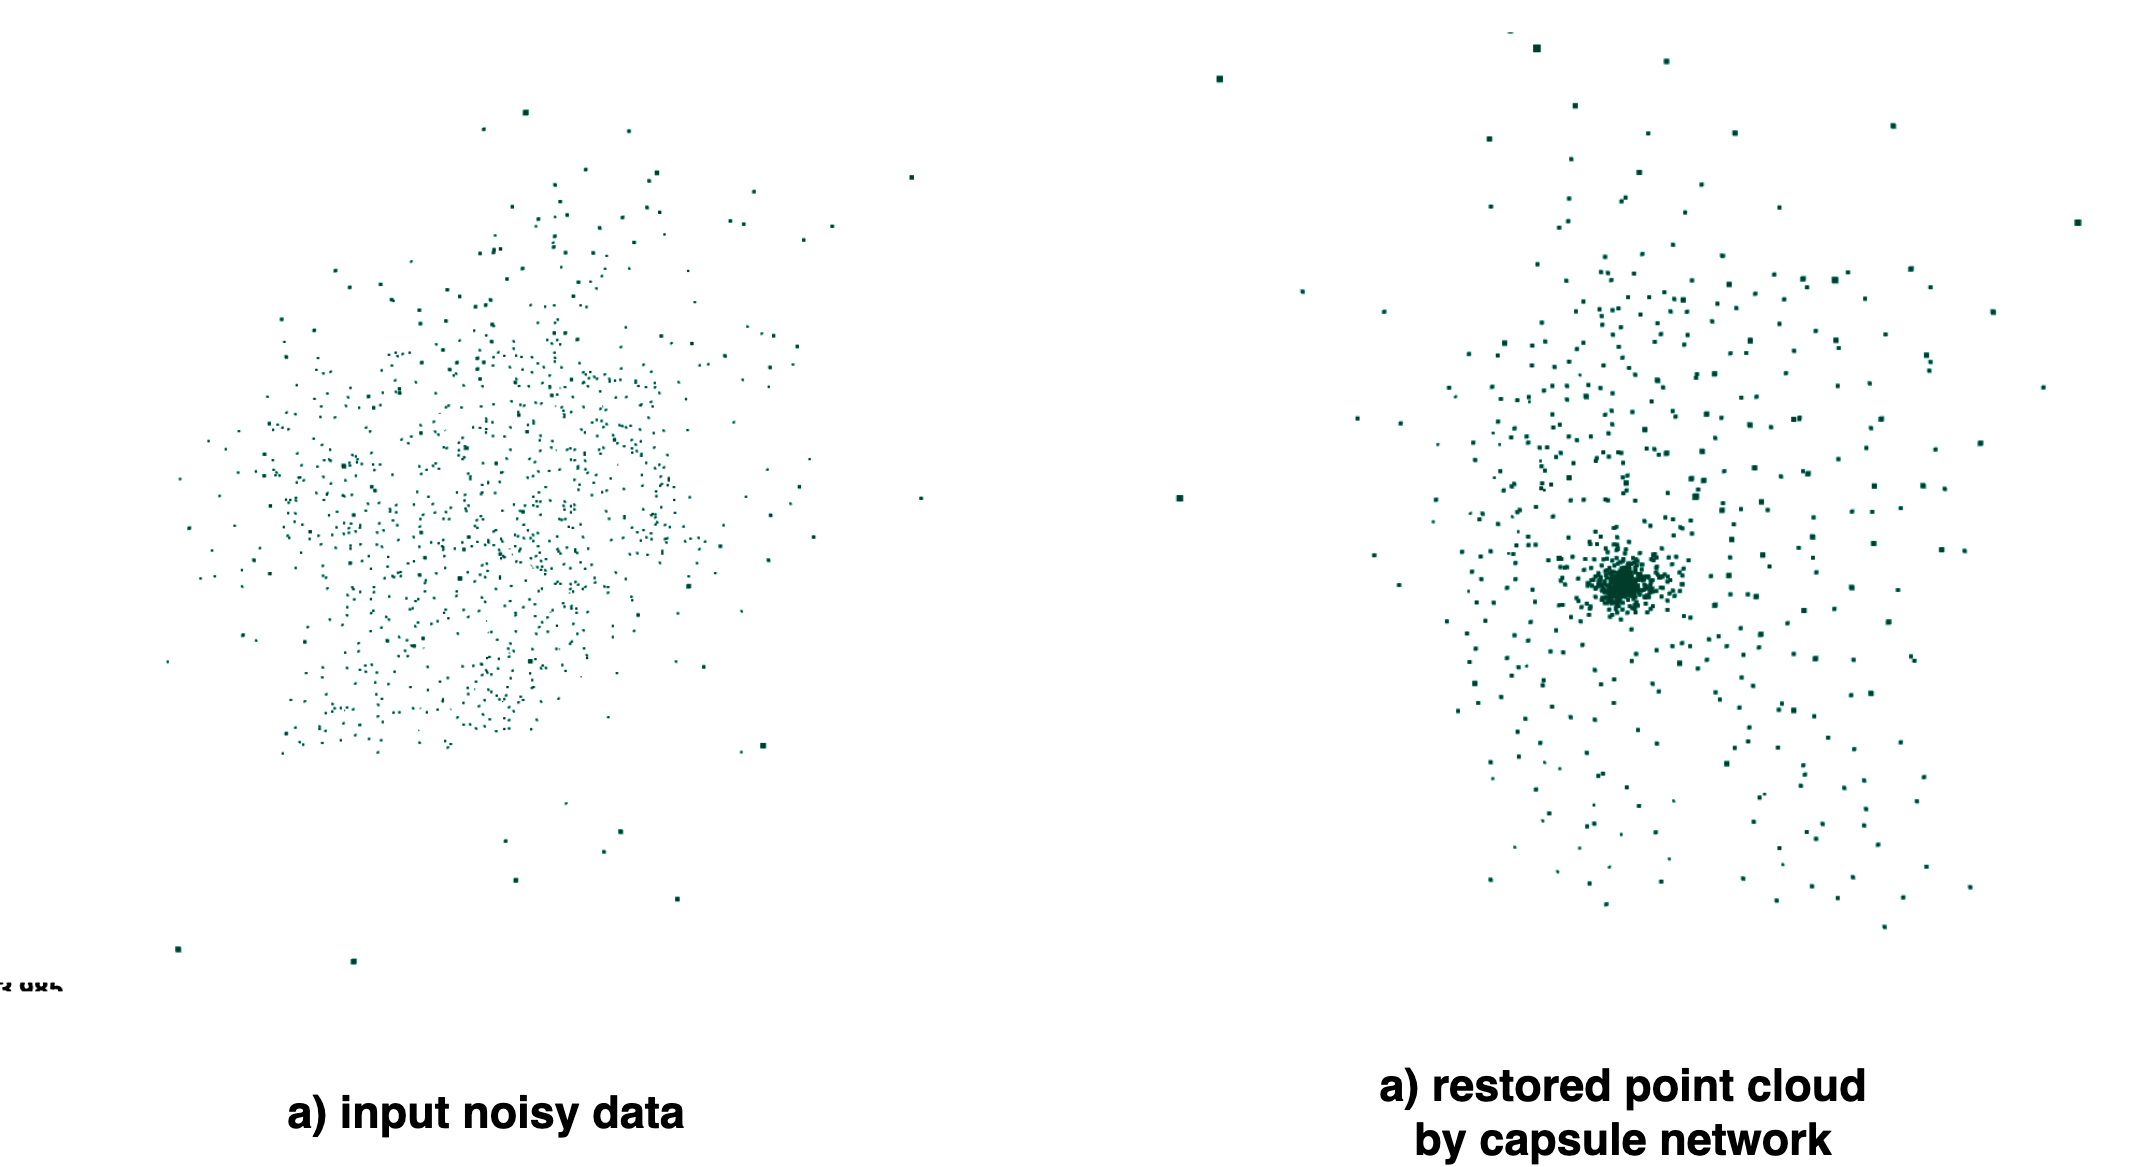
\includegraphics[scale=0.2]{Figures/noise-resporation.png}}
    \caption{Example of noisy point cloud (left), and restored point cloud by capsule network (left)}
    \label{img:denoising}
\end{figure}

Based on the visual analysis we could say that a capsule-based network filters the majority amount of noisy data and potentially could be used as a denoiser.

\section{Models' performance with the lack of data}
\label{s:experiment-lack-of-data}
In this section, we evaluate the capsule-based model with different amounts of training data. Also, we compare the performance with the SOTA model - PoseNet.

For the capsule-based model, we run training pipelines with different training dataset sizes (16/16 as a reference, 15/16, 12/16, and 8/16). The pipeline setup is described in Section~\ref{s:experiment-setup}. After each run of training, we measure the mAP for 10 cm distance on the test dataset.

For PoseNet we use the same approach of retraining the model with different train sizes. The training code was used from the original\footnote{\url{https://github.com/mks0601/V2V-PoseNet_RELEASE}} implementation of the model. Also, we use default parameters for the PoseNet network.

As a benchmark dataset, we use the ITOP side view.

The comparison table for the set of experiments could be found in Table~\ref{tab:truncated-data}.

\begin{table}[H]
    \caption{The comparison of capsnet model and PoseNet trained on different amound of data (ITOP side view)}
    \label{tab:truncated-data}
    \centering
    \begin{tabular}{l l l l l}
    \toprule
    \tabhead{Dataset size} & \tabhead{PoseNet} & \tabhead{CapsNet} & \tabhead{PoseNet difference} & \tabhead{CapsNet difference}  \\
    \midrule
    $16/16$ (full dataset) & 86.2\%  & 83.1\%  & 0\% & 0\% \\
    $15/16$ & 86.0\%  & 82.8\%  & 0.2\% & 0,3\% \\
    $12/16$ & 80.2\%  & 74.3\%  & 6,0\% & 8,8\% \\
    $8/16$ & 63.7\%  & 56.0\%  & 30,2\% & 27,1\% \\
    \bottomrule\\
    \end{tabular}
\end{table}

As we can see from the results capsule-based model underperform compared to PoseNet model. The only experiment where the capsule-based model shows a better mAP difference is the case with 8/16 of the dataset. In this experiment capsule model shows $27,1\%$ of mAP drop compared to $30,2\%$ in PoseNet.

Taking everything into account we can't prove a hypothesis that a capsule-based network works better in data lack environment compared to another SOTA model. However, this statement is hold only for current experiment setup and could change on other datasets.